\documentclass[12pt,a4paper]{article}

\usepackage{float}
\restylefloat{figure}
\usepackage{hyperref}
\usepackage{graphicx}
\usepackage{gensymb}
\usepackage[title]{appendix}
\usepackage[dotinlabels]{titletoc}
\usepackage[nottoc,numbib]{tocbibind}
\usepackage{mathtools}
\usepackage[margin=0.5in]{geometry}
\renewcommand{\thefootnote}{\arabic{footnote}}

\newcommand*\wrapletters[1]{\wr@pletters#1\@nil}
\def\wr@pletters#1#2\@nil{#1\allowbreak\if&#2&\else\wr@pletters#2\@nil\fi}

\usepackage{enumitem}
\setenumerate{itemsep=0pt}

% Add support for multi-page tables.
\usepackage{longtable}

\pagenumbering{arabic}

\title{EE4DSA Coursework 2}
\author{Chris Cummins}

\begin{document}
\maketitle

\section{Disassembling the program ROM}

The file \texttt{extra/rom.asm} contains a heavily annotated
disassembled version of the safe unlocking program, in a style
inspired by the AVR Assembler Syntax. The program tests for the safe
code 4D5A.

The assembly code was generated automatically using a disassembler
developed for this purpose, available at
\url{http://chriscummins.cc/disassembler}. Based off of the
implementation for the first coursework disassembler, the
functionality has been extended to support the subroutine and
interrupt instructions, and development effort has been focused on
making the output easier to understand.

Generated label names now distinguish between subroutines, interrupt
handlers and sections, and the UI now supports syntax highlighting,
automatic comment generation, line highlighting and jumping to
sections (clicking on a branch or jump instruction will now take the
user to the specific address). Backwards compatibility with the first
coursework instruction set is ensured by allowing the user to select
between an initial program counter of either 0x00 or 0x08.

\begin{figure}[H]
  \centering
  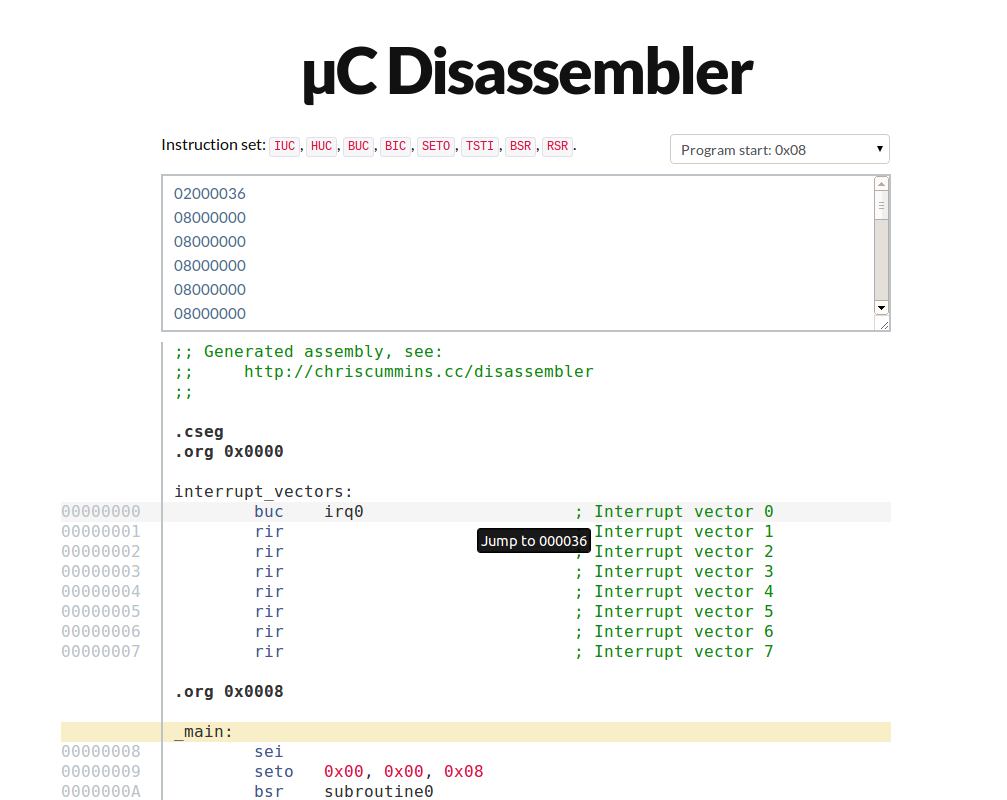
\includegraphics[width=6.2in]{assets/disassembler.png}
\end{figure}

The disassembler is implemented in 479 lines of JavaScript, with the
source code available at\\*
\url{http://chriscummins.cc/js/disassembler.js}.

\section{Modifying the ROM program}

The file \texttt{rom.dat} contains a modified ROM program which uses
the last four digits of my SUN number (5189) as the code to the
safe. The only modifications required were to the \texttt{AND}
components of the four \texttt{TSTI} instructions. The
\texttt{test\_bench\_inputs.dat} file was then modified so as to test
this new code.

\section{Implementing the Execution Unit}

The file \texttt{execution\_unit.vhd} contains my implementation of
the instruction set. The execution unit uses three processes, with two
multiplexers controlling the next values for program counter and
status registers.

%% TODO: Max frequency, and longest paths. (2 processes would be
%% faster). Mention the big refactor for .5Mhz increase.

A video demonstration of the program can be found at
\url{http://youtu.be/TODO}, showing how the program behaves when
inputting a correct code, invalid code, and interrupting normal
program behaviour by resetting the board.

\end{document}
